\documentclass[conference]{IEEEtran}
\IEEEoverridecommandlockouts
% The preceding line is only needed to identify funding in the first footnote. If that is unneeded, please comment it out.
\usepackage{cite}
\usepackage{amsmath,amssymb,amsfonts}
\usepackage{algorithmic}
\usepackage{graphicx}
\usepackage{textcomp}
%\usepackage{subcaption}
\usepackage{natbib}
\usepackage{float}
\usepackage{xcolor}
\usepackage{authblk}
\bibliographystyle{plainnat}
\def\BibTeX{{\rm B\kern-.05em{\sc i\kern-.025em b}\kern-.08em
    T\kern-.1667em\lower.7ex\hbox{E}\kern-.125emX}}


\title{Machine Learning Based Approaches to Accurate Diamond Price Prediction\\
\thanks{Final Project Report ECS-171: \textbf{Group 21}}
}

% \author{
% \IEEEauthorblockN{Aditya Mittal}
% \IEEEauthorblockA{\textit{Department of Statistics} \\
% \textit{University of California, Davis}\\
% Davis, United States \\
% adimittal@ucdavis.edu}
% \and
% \IEEEauthorblockN{Andrew Yeow}
% \IEEEauthorblockA{\textit{Department of Computer Science} \\
% \textit{University of California, Davis}\\
% Davis, United States \\
% XXX}
% \and
% \IEEEauthorblockN{Yifan Cui}
% \IEEEauthorblockA{\textit{Department of Computer Science} \\
% \textit{University of California, Davis}\\
% Davis, United States \\
% harcui@ucdavis.edu}
% \and
% \IEEEauthorblockN{Nandini Koladi}
% \IEEEauthorblockA{\textit{Department of Computer Science} \\
% \textit{University of California, Davis}\\
% Davis, United States \\
% XXX}
% \and
% \IEEEauthorblockN{Eshan Toshniwal}
% \IEEEauthorblockA{\textit{Department of Computer Science} \\
% \textit{University of California, Davis}\\
% Davis, United States \\
% XXX}
% }

\author[1]{Aditya Mittal}
\author[2]{Andrew Yeow}
\author[3]{Yifan Cui}
\author[4]{Nandini Kodali}
\author[5]{Eshan Toshniwal}
\affil[1]{Department of Statistics; University of California, Davis}
\affil[2]{Department of Computer Science; University of California, Davis}
\affil[3]{Department of Computer Science; University of California, Davis}
\affil[4]{Department of Computer Science; University of California, Davis}
\affil[5]{Department of Computer Science; University of California, Davis}

\begin{document} 
\maketitle

\begin{abstract}
In 2023, the U.S. jewelry market was valued at an approximate 73.32 billion USD, with diamonds capturing a significant share. Consequently, accurate diamond price prediction of diamonds is critical for both jewelers and consumers alike. This paper explores several machine learning algorithms, including regression models, tree-based ensemble methods, and artificial neural networks, to predict diamond prices based on important characteristics such as carat, cut, color, and clarity. Our exploratory data analysis identified carat as the most influential feature with regards to diamond prices. Our methodology involves rigorous model evaluation using metrics like Mean Squared Error (MSE), Mean Absolute Error (MAE), and R-squared ($R^2$) on testing data. The experimental results indicate that \emph{XGBoost} outperformed other models by achieving the lowest testing error, followed closely by Random Forests and the Artificial Neural Network. Polynomial regression also performed well, capturing the non-linear relationship between diamond prices and its features. The neural network model also demonstrated strong results for predictions, and will benefit from further tuning. By developing a robust predictive model, we aim to enhance pricing precision, benefiting both businesses and consumers in the diamond market.
\end{abstract}

\begin{IEEEkeywords}
Diamond Pricing, Machine Learning, Artificial Neural Network, Ensemble Methods - Random Forests, XGBoost
\end{IEEEkeywords}

\section{Introduction}

In 2023, the jewelry market in the United States was estimated to be worth 73.32 billion USD, with projections for 2024 reaching 96.61 billion USD \cite{us}. Clearly, the market for jewelry is quite significant and continues to display steady growth. In particular, \emph{diamonds} account for a significant portion of this market, covering an estimated 50-60\% market share as compared to some of the other precious stones such as gold, silver, etc \cite{diamond}. Consequently, it becomes important for jewelers to adopt accurate methods to predict prices of these diamonds to better serve their consumers. In fact, businesses have began educating their sellers on essential qualities such as cut, color, carat weight, and clarity to make informed pricing decisions. As such, ensuring accurate price predictions becomes very important as it has significant financial implications on both businesses and consumers alike. Figure \ref{fig:diamond_intro} below demonstrates the importance of accurate diamond pricing. Two diamonds can differ significantly based on features such as carat, underscoring the need for precise price prediction methods. 

\begin{figure}[H]
    \centering
    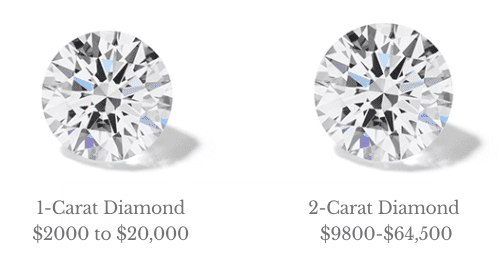
\includegraphics[width=0.8\linewidth]{diamond_intro.png} % Replace "example-image" with the filename of your image
    \caption{Two different diamonds differing in carat and overall pricing. The 1-carat diamond ranges from \$2,000- \$20,000, while the 2-carat diamond ranges from \$9,800 to \$64,500. This highlights the importance of accurate price prediction based on the given characteristics.}
    \label{fig:diamond_intro}
\end{figure}

Given the importance of this task, it becomes crucial to develop methods that enable accurate prediction of prices for these diamonds. Machine learning, with its ability to learn patterns in data and generate predictions, has become extremely popular in recent years across a wide range of applications \cite{kino}. Recent advancements in machine learning have introduced a range of algorithms, including linear regression, K-Nearest Neighbors, Random Forests, and the increasingly popular neural networks \cite{sarker}. In this paper, we explore several different machine learning algorithms to accurately predict diamond prices based on their given characteristics, including those mentioned above. The application of creating models to generate accurate predictions is widespread, as it can aid jewelers and marketers who aim to provide accurate pricing methods for consumers in the jewelry market.

Our dataset contains several essential features for diamond price prediction, such as the aforementioned carat, cut, color, clarity, etc. \cite{kaggle} Through exploratory data analysis (EDA), we aim to understand how these features are related to diamond pricing. This analysis will help us answer questions about which features most significantly impact diamond prices and ways we can leverage this information to create accurate predictive models. Ultimately, our goal is to develop an accurate model for predicting diamond prices, enabling jewelers to make precise pricing decisions and improve the overall consumer purchasing experience. This paper details our methodology, including EDA and the application of various machine learning algorithms, to achieve this objective.

The outline of this paper is as follows: Section 2 reviews the related literature on diamond price prediction and provides a historical perspective on machine learning and relevant algorithms. Section 3 presents data description and exploratory data analysis. Sections 4 and 5 highlight the proposed methodology and results. Finally, the paper concludes with a discussion and future perspective in Section 6.

\section{Literature Review}

Much literature has been published to develop predictive models for accurately estimating diamond prices, using various social contexts and individual diamond characteristics. Alsuraihi et al. \cite{Alsuraihi} aimed to develop an accurate algorithm to estimate diamond prices. They considered various features such as diamond sizes and other key factors. Various machine learning methods were tested, including Linear Regression, Random Forest Regression, Polynomial Regression, Gradient Descent, and Neural Networks. Similarly, Mamonov and Triantoro \cite{Mamonov} studied the relationship between a diamond's physical attributes and respective prices in e-commerce contexts, with the goal of understanding how these attributes affect diamond prices. However, their study did not account for the diamond cut – a significant factor affecting market value – which is indeed included in our dataset. Pandey et al. \cite{Pandey} addressed the challenge of forecasting future values of precious metals like gold and diamonds. They used ensemble approaches combined with feature selection techniques to enhance prediction accuracy. In an alternate perspective, Scott and Yelowitz \cite{Scott} investigated diamond prices in the context its social status and intrinsic value. They collected data from online diamond sellers and empirically examined factors influencing diamond prices, considering carat weight, color, cut, and clarity in determining the logarithm of price. Clearly, a variety of approaches have been taken to create accurate prediction models, ranging from investigating social contexts to individual characteristics. In this paper, we utilize several algorithms to create accurate models and build on this previous work. With this, the latter half of this section provides an overview of several machine learning algorithms applied in this paper, including regression models, decision trees, and neural networks. We also examine Grid Search as a method for hyperparameter tuning.

\subsection{Linear Regression}

Linear regression is one of the simplest and one of the most interpretable prediction models. It fits a straight line between the response variable $Y$ and its predictors $X$. The goal of this model is to minimize the Residual Sum of Squares (RSS) \cite{Seber}:

\[
\text{RSS} = \sum_{i=1}^n (y_i - \hat{y}_i)^2
\]

Linear regression requires several assumptions: linearity, independence, homoscedasticity, and normality of residuals \cite{Kutner}. Its performance may be  evaluated using metrics like $R^2$, Mean Squared Error (MSE), Mean Absolute Prediction Error (MAE). Extensions include multiple linear regression, polynomial regression, and regularization methods like Ridge and Lasso regression to handle complex relationships and handle overfitting \cite{Wright, Weisberg}.

\subsection{Decision Trees}

Decision trees are very effective on tabular data, as they display strong performance on both regression and classification tasks. These models split the data based on feature values, forming a tree-like structure. In particular, decision trees are prone to overfitting. Ensemble methods, such as Random Forests \cite{Breiman} and Gradient Boosting Machines like XGBoost \cite{Chen}, mitigate this issue by combining multiple trees, thereby enhancing performance and robustness of these methods.

\subsection{Neural Networks}

Neural networks have recently become extremely popular with advances in deep learning and computation ability to handle big data problems \cite{LeCun}. These models consist of layers of interconnected nodes (neurons) that learn representations from data. In forward propagation, input data traverses through neural network layers, where each layer applies weights and passes results through activation functions, crucial for introducing nonlinearity. Activation functions like ReLU facilitate this nonlinearity, enabling neural networks to learn complex patterns and relationships in data, enhancing their effectiveness in various tasks. To learn the model weights, Rumelhart et. al \cite{Rumelhart} introduced the backpropagation algorithm by iteratively minimizing the training loss across each epoch. SGD (Stochastic Gradient Descent) is a foundational optimizer that updates parameters in the direction of the negative gradient of the loss function, often with momentum to accelerate convergence \cite{Bottou}. Modern neural networks use optimizers like Adam (Adaptive Moment Estimation), which combines adaptive learning rates and momentum for efficient training \cite{Kingma}. RMSprop (Root Mean Square Propagation) is another popular optimizer in modern neural networks, which adaptively scales the learning rate for each parameter based on the magnitude of recent gradients \cite{Tieleman}. We test each of these optimizers when finding the optimal set of hyperparameters of our neural network model. 

\subsection{Grid Search}

Both Neural Networks and decision trees include a variety of hyperparameters that significantly impact their performance and overall generalization ability on unseen data. In the context of decision trees, important hyperparameters include the maximum depth of the tree, minimum samples required to split a node, and the minimum samples required at each leaf node. For neural networks, key hyperparameters encompass the learning rate, batch size, number of hidden layers, and the number of neurons per layer. Grid search is a method for hyperparameter tuning that evaluates a predefined set (grid) of hyperparameters and finds the optimal configuration among them. This method is quite computationally heavy, as it explore every configuration among the given hyperparameter space to identify the most suitable combination for a given problem. Bergstra and Bengio (2012) \cite{Bergstra} discusses grid search's efficiency and limitations highlights its importance in fine-tuning machine learning models for optimal performance.

With this, our literature review provides a comprehensive overview of the previous efforts conducted on predicting diamond prices, including discussions on pertinent algorithms such as linear regression, decision trees, and neural networks. For hyperparameter tuning, we plan to utilize Grid Search to optimize the performance of both the decision trees and neural network models. Next, we proceed with dataset exploration and perform pre-processing on our features.

\section{Dataset Description and Exploratory Data Analysis}

The \emph{diamond prices} dataset contains detailed information about 54,000 diamonds, including their prices and various characteristics \cite{kaggle}. The predictor variables in this dataset are as follows: i) \textbf{Carat}: Represents the weight of the diamond, ranging from 0.2 to 5.01 carats. ii) \textbf{Cut Quality}: Categorized as Fair, Good, Very Good, Premium, or Ideal, indicating the craftsmanship involved in shaping the diamond. iii) \textbf{Color}: Graded from J (worst) to D (best), reflecting the hue and saturation of the stone. iv) \textbf{Clarity}: Measures how clear the diamond is, with grades ranging from I1 (worst), SI2, SI1, VS2, VS1, VVS2, VVS1, to IF (best). v) \textbf{Dimensions}: Captured by the length (x), width (y), and depth (z) in millimeters, with ranges of 0–10.74 mm, 0–58.9 mm, and 0–31.8 mm, respectively. vi) \textbf{Depth Percentage}: Ranges from 43\% to 79\%. vii) \textbf{Table}: Represents the width of the top of the diamond relative to its widest point, ranging from 43\% to 95\%. The dataset does not contain any missing values, so we do not need to any address missing data in the exploratory data analysis step.

\subsection{Exploratory Data Analysis}

To explore the dataset further and understand the relationships between these features and diamond prices, we will conduct exploratory data analysis (EDA). First, we visualize the distribution of each continuous feature, such as carat, length (x), width (y), depth (z), depth percentage, and table, to understand their spread and central tendencies. A table will highlight the mean, median, and standard deviation statistics of each feature, providing insights into their individual magnitudes and spread. Second, pairwise scatter plots display the relationship between each continuous feature and diamond price, helping to identify potential trends and correlations. Third, the correlation heat-map presents Pearson correlation relationships between continuous features, helping identify features most correlated with price. Finally, we create histograms of categorical features like cut, color, and clarity to understand their distributions. These visualizations provide insights into the structure of the data, highlight any anomalies, and help with subsequent modeling efforts to predict diamond prices effectively.

\begin{figure}[H]
    \centering
    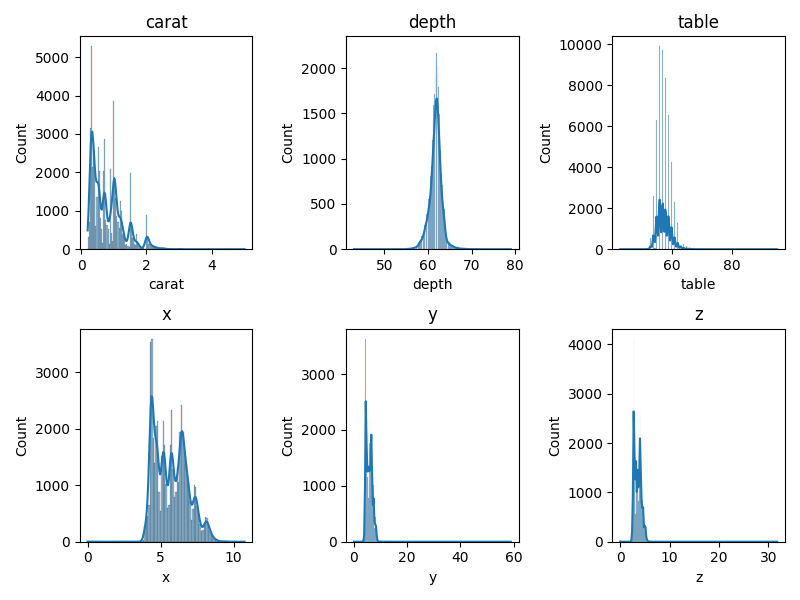
\includegraphics[width=0.60\linewidth]{distribution_plots.png}
    \caption{Distribution Plot of Continuous Features. Identify trends in our dataset such as skewness, location of outliers, mean, median, scale, etc.}
    \label{fig:distribution}
\end{figure}

Figure \ref{fig:distribution} displays the distribution of continuous predictors and highlight potential skewness in our dataset. For instance, the predictor \emph{carat} suggests potential skewness to the right – with many upper outliers – as evidenced by its distribution plot. This trend holds true for features \emph{y} and \emph{z} as well. These plots suggest that our dataset may contain a significant number of upper outliers, which we will consider removing in the data pre-processing stage. To further gain insight on the distribution of our continuous features, the table below summarizes the mean, median, and standard deviation of the each predictor:

\begin{table}[H]
    \centering
    \caption{Mean, Median, Standard Dev. of Continuous Features}
    \label{tab:example_table}
    \begin{tabular}{|c|c|c|c|}
        \hline
        Feature & Mean & Median & Standard Dev. \\
        \hline
        Carat & 0.797 & 0.70 & 0.474 \\
        \hline
        Depth & 61.749 & 61.80  & 1.432 \\
        \hline
        Table & 57.457 & 57.00 & 2.234 \\
        \hline
        X & 5.731 & 5.70 & 1.122 \\
        \hline
        Y & 5.734 & 5.71 & 1.142 \\
        \hline
        Z & 3.538 & 3.53 & 0.705 \\
        \hline
    \end{tabular}
\end{table}

From our table, we can observe that the mean and median values for most features are relatively close, indicating that the data distributions may not actually be as heavily skewed for most variables. However, the standard deviation values highlight the variability within each feature, such as carat and dimensions (x, y, z), display considerable spread. This variability and potential skewness (from the plots), especially in the carat feature from the plots, could influence our predictive algorithms. Next, we will create pairwise scatter-plots to identify trends between diamond prices and the features.

\begin{figure}[H]
    \centering
    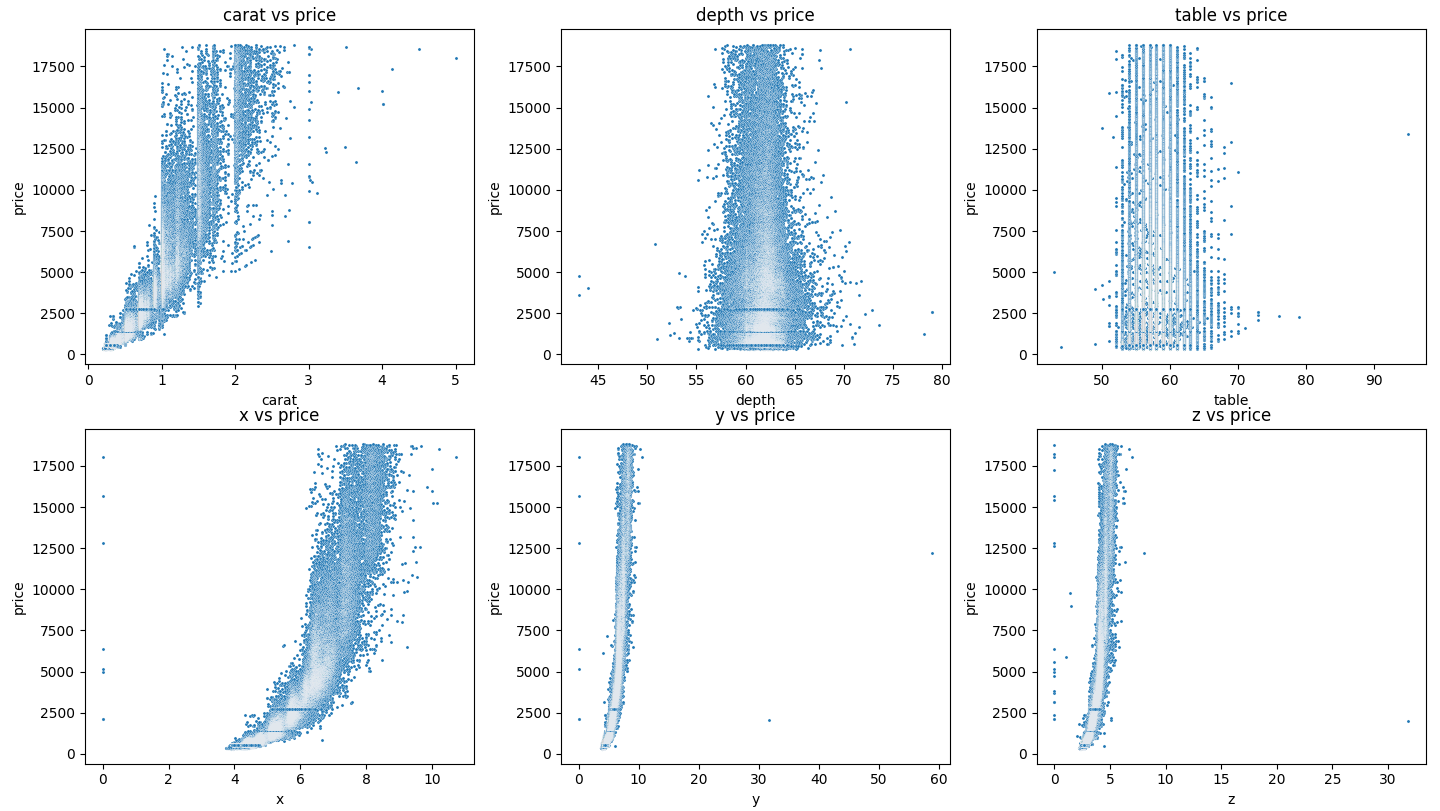
\includegraphics[width=0.61\linewidth]{scatter.png} 
    \caption{Pairwise scatter-plots for Each Feature vs. Diamond Price. Displays a quadratic relationship between Carat, x, y, z and diamond pricing.}
    \label{fig:scatter}
\end{figure}

Figure \ref{fig:scatter} displays the scatter-plots of each feature against the response variable, we observe a quadratic relationship between the features, carat, x, y, and z, with respect to the the response variable price. This suggests that a polynomial regression model might be suitable for our dataset in addition to a linear regression model. Thus, we will evaluate the polynomial regression model's performance on this dataset and compare it with traditional linear regression. Next, we will analyze the correlations between the continuous features and the target variable, price, to determine the most influential predictors. This will allow us to identify the most relevant features and potential multicollinearity and interactions among the predictors.

\begin{figure}[H]
    \centering
    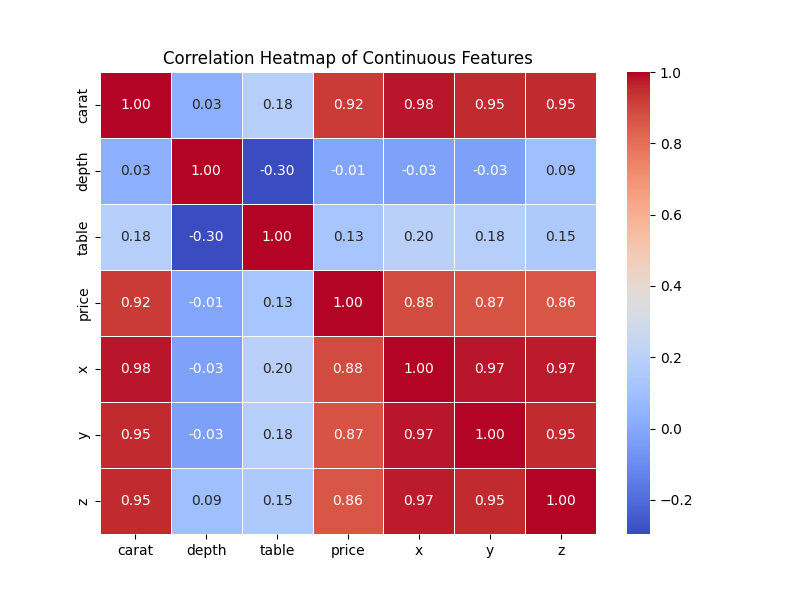
\includegraphics[width=0.7\linewidth]{correlation.png} % Replace "example-image" with the filename of your image
    \caption{Correlation Heat-Map for Continuous Features vs Diamond Price. It reveals that the feature 'carat' has the highest correlation (0.92) with diamond pricing.}
    \label{fig:corr}
\end{figure}

Based on the results of our correlation heatmap in figure \ref{fig:corr}, the feature \emph{Carat} appears to be highly correlated with price, with a correlation coefficient of 0.92. Similarly, it is correlated with dimension features \emph{x}, \emph{y}, and \emph{z}. This makes sense, as carat weight would directly relate to diamond size. Thus, this plot suggests that Carat (and potentially dimensions) are the strongest predictors for diamond price. On the other hand, both depth percentage and table have almost zero correlation, indicating that they do not have much association with diamond prices. We showcase data pre-processing methods for outlier removal using carat below. Thus, this heatmap is insightful in identifying the key predictors for diamond prices and guiding our feature selection process. Next, we will examine histograms for the distribution of categorical features cut, clarity, and color:

\begin{figure}[H]
    \centering
    \includegraphics[width=0.8\linewidth]{histogram.png} 
    \caption{Histogram for the distribution of categorical features: Cut, Clarity, and Color.}
    \label{fig:histogram}
\end{figure}

The histogram of the categorical variables displays their frequencies. Upon initial analysis of the plot, we observe that the cut category "Ideal" appears most frequently, followed by "Premium" and "Very Good," while the "Fair" cut appears least frequently. The distribution of color appears to be well spread, with all colors represented. Regarding clarity, categories such as "I1" and "IF" have relatively few observations compared to others. With this, our exploratory data analysis step has provided valuable insights into the structure of the dataset and identify patterns among the features. We will now proceed with data pre-processing before implementing our machine learning algorithms.

\subsection{Data Pre-Processing} 

Before implementing the machine learning algorithms, we conducted several pre-processing steps on our dataset. First, considering the ordinality present in each of our categorical features, we implemented label encoding to convert these features into numeric representations. The mappings for each categorical feature were defined as follows:

\begin{table}[htbp]
    \centering
    \caption{Label Encodings for Categorical Features}
    \resizebox{\columnwidth}{!}{
        \begin{tabular}{|l|l|}
            \hline
            \textbf{Feature} & \textbf{Encoding} \\
            \hline
            Cut & 'Fair': 0, 'Good': 1, 'Very Good': 2, 'Premium': 3, 'Ideal': 4 \\
            Color & 'J': 0, 'I': 1, 'H': 2, 'G': 3, 'F': 4, 'E': 5, 'D': 6 \\
            Clarity & 'I1': 0, 'SI2': 1, 'SI1': 2, 'VS2': 3, 'VS1': 4, 'VVS2': 5, 'VVS1': 6, 'IF': 7 \\
            \hline
        \end{tabular}
    }
    \label{tab:label_encodings}
\end{table}

Next, to standardize our data and balance the scale of our features, we applied z-score transformation. This transformation ensures that all our features have a mean of 0 and a standard deviation of 1, thereby balancing the scales among features. This is particularly beneficial for algorithms such as neural networks. Finally, we proceeded to remove outliers. Since carat was our most highly correlated predictor, we used it as the feature to identify and remove outliers using the 1.5 times the interquartile range (IQR) calculation. Approximately 3.9\% of the dataset was removed through this process, leaving us with 51,800 rows of data. The boxplots for each feature post outlier removal are shown below:

\begin{figure}[H]
    \centering
    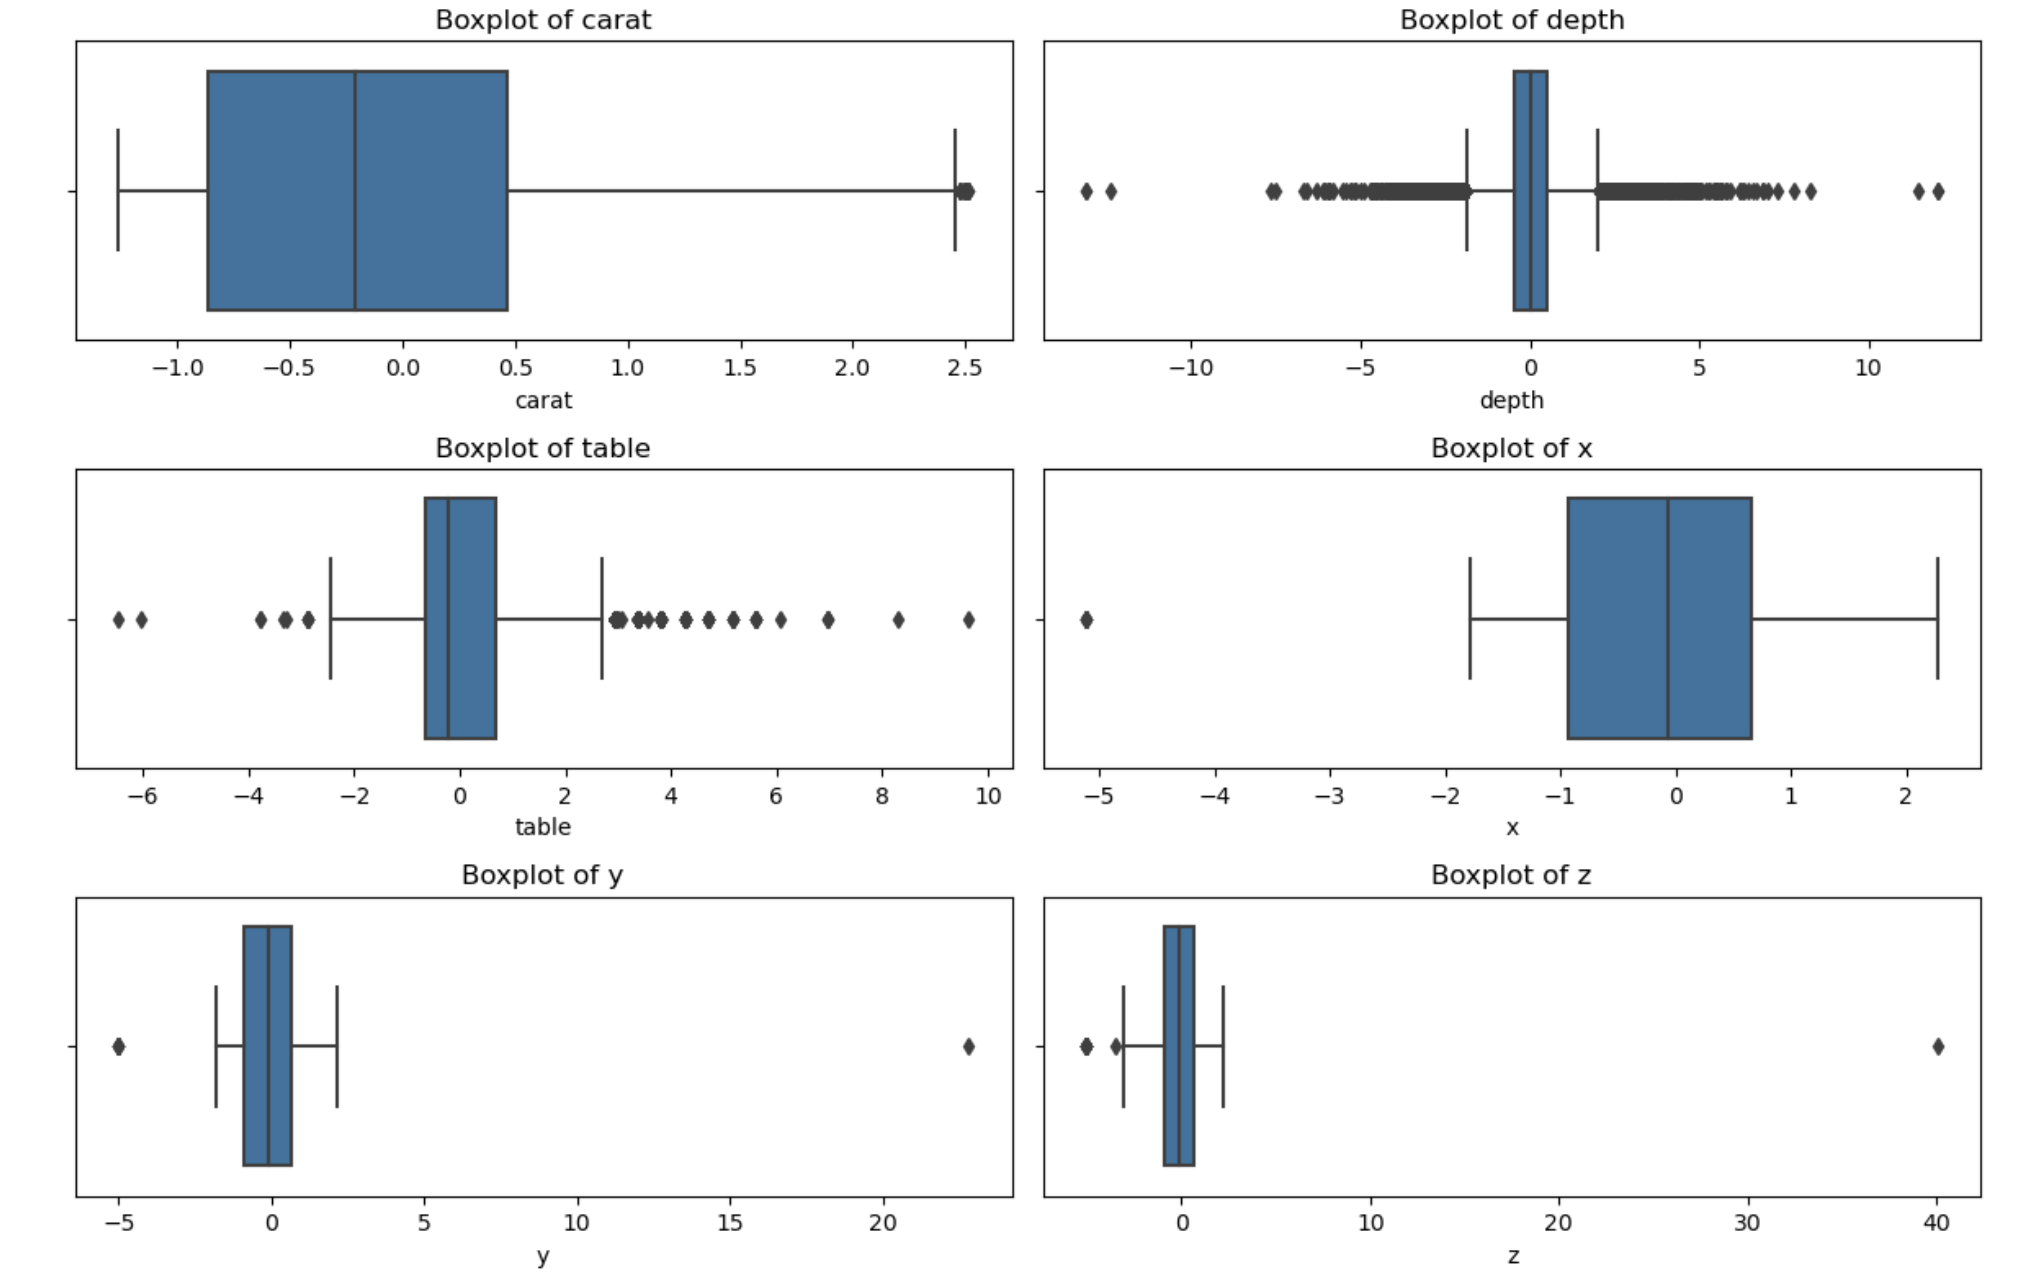
\includegraphics[width=0.8\linewidth]{boxplot.png} % Replace "example-image" with the filename of your image
    \caption{Boxplots of Features Post-Outlier Removal}
    \label{fig:boxplots}
\end{figure}

The boxplots indicate that outliers were removed for carat, while several other features such as depth and table still exhibit upper values. Since these features are not highly correlated with our response variable, we decided to keep them as is and proceed with this cleaned version of the dataset. 

\section{Proposed methodology}

In this paper, we will implement various machine learning algorithms to generate accurate diamond predictions. The models will include linear regression, decision trees, and artificial neural networks. Our approach involves several steps to develop and evaluate model performance to choose the best algorithm for this application. Data preprocessing has been completed as described earlier. The dataset has been divided into training and testing sets using a 75:25 split. The training data comprises 38,200 rows, while the testing data contains approximately 12,800 rows. We apply cross-validation procedures (detailed below) on our training data to determine the optimal degree of our polynomial regression model and the optimal set of hyperparameters for the decision trees and neural network models.

\subsection{Regression Models}

We begin with the simplest algorithm: the Linear regression model. This algorithm fits a straight-line model between diamond prices and the aforementioned features. This initial model will help us gain intuition about the relationship between the features and diamond prices. Additionally, since our results in \ref{fig:scatter} suggested a potential quadratic relationship between price and carat \& diamond dimensions (x, y, z), we also implement a Polynomial Regression model and test its performance. Using 5-fold cross-validation, we test powers ranging from 1 to 3 to determine the optimal degree of our regression model. This allows us to identify whether more complex relationships in our data exist, capture nonlinear relationships, and assess whether Polynomial Regression outperforms traditional Linear Regression. After determining the optimal degree of our polynomial regression model, we will train the algorithm on the entire training dataset. Finally, we evaluate its performance on the test set to compare it with other algorithms.

\subsection{Decision Trees} 

For decision tree-based models, we implement two algorithms: Random Forests and XGBoost. Random Forests aggregate the predictions of multiple decision trees to enhance accuracy and reduce overfitting; XGBoost is a gradient boosting algorithm that iteratively optimizes the model to minimize overall error. To determine the optimal set of hyperparameters for each algorithm, we employ grid search with 5-fold cross-validation on our training data. The following sets of hyperparameters were tested for each algorithm:

\begin{itemize}
    \item \textbf{Random Forests}: 
    \begin{itemize}
        \item \emph{Bootstrap}: True
        \item \emph{Max\_features}: 'auto' and 'sqrt'
        \item \emph{Max\_depth}: None, 5, and 10
        \item \emph{Min\_samples\_leaf}: 1 and 2
        \item \emph{Min\_samples\_split}: 1 and 2
        \item \emph{N\_estimators}: 1, 5, and 10
    \end{itemize}
    
    \item \textbf{XGBoost}: 
    \begin{itemize}
        \item \emph{Max\_depth}: 3, 6, and 9
        \item \emph{Learning\_rate}: 0.1 and 0.01
        \item \emph{N\_estimators}: 100, 200, and 300
        \item \emph{Subsample}: 0.8 and 1.0
        \item \emph{Colsample\_bytree}: 0.8 and 1.0
        \item \emph{Gamma}: 0 and 0.1
        \item \emph{Reg\_alpha}: 0 and 0.1
        \item \emph{Reg\_lambda}: 0 and 0.1
    \end{itemize}
\end{itemize}

Using grid search, we explore various hyperparameter values to assess different model configurations and identify the optimal combination for our dataset. This comprehensive approach allows us to evaluate both simple and complex models, informing us about the algorithm configuration that yields the most accurate predictions. Subsequently, we train the model using these optimized hyperparameters on the training data and evaluate its performance on the testing set. We compare results with the regression and neural network models.

\subsection{Neural Networks}

Our final model being testing is an artificial neural network. The architecture consists of a single hidden layer with ReLU activation, followed by an output layer also using ReLU activation, given our regression task. The hyperparameters explored during grid search are found using a 5-fold cross-validation procedure on our training data; these include learning rate, batch size, optimizer, dropout rate, and the number of neurons in the hidden layer. Through this process, we will identify the optimal configuration of hyperparameters that maximizes the predictive performance of our neural network model on the given dataset. We explore the following set of hyperparameters:

\begin{itemize}
    \item \emph{Learning Rate:} 0.001, 0.01, 0.1
    \item \emph{Batch Size:} 256, 512, 1028
    \item \emph{Optimizer:} rmsprop, adam, SGD
    \item \emph{Dropout Rate:} 0, 0.2, 0.5
    \item \emph{Number of Neurons in Hidden Layer(s):} 16, 32, 64
\end{itemize}

This comprehensive exploration of hyperparameters will provide insights into the set of hyperparameters that give the best results. We will evaluate the impact of different learning rates and batch sizes on the model convergence, while adjusting the number of hidden layers and dropout rates manage model complexity and implement potential regularization in the hidden layer. As shown above, we test the three different optimizers of our neural network model to achieve the best performance on this dataset with the corresponding hyperparameters. By evaluating these hyperparameters, our aim is to optimize the neural network model's performance and improve its predictive accuracy for the given diamond dataset.

\subsection{Evaluating Model Performance}

To identify the optimal hyperparameters in our grid search, we will use the \emph{negative mean squared error} as our evaluation metric for both decision trees and the artificial neural network. With this metric, we aim to determine the best set of hyperparameters for each model. We will subsequently train the models using these optimal hyperparameters on the entire training data. To assess model performance on the testing data and compare the algorithms, we will compare results using various metrics, including Mean Squared Error (MSE), Mean Absolute Error (MAE), and R-squared ($R^2$). These metrics offer a comprehensive understanding of model performance, aiding in evaluating accuracy and fit. Additionally, we will display the training time for each model, providing insight into computational complexity. This evaluation process aims to identify the most effective algorithm for predicting diamond prices, offering valuable insights for both jewelers and consumers in the industry. For jewelers, accurate price predictions enable better inventory management and pricing strategies, while consumers benefit from informed purchasing decisions. Through this methodology, we aim to develop an accurate model for predicting diamond prices, leveraging the strengths of various machine learning techniques to achieve the best possible performance.

\section{Experimental results and evaluation}

In this section, we present our experimental results where we evaluated the performance of each machine learning algorithm. Through this analysis, we aim to demonstrate the effectiveness and suitability of each approach, offering valuable insights for deploying commercial algorithms in predicting diamond prices.

\subsection{Linear \& Polynomial Regression}

As previously mentioned, we've implemented both multiple linear regression and polynomial regression models using all available features in our dataset. During the exploratory data analysis (EDA) phase, we observed a possible quadratic relationship between diamond prices and the predictors as shown in Figure \ref{fig:scatter}. However, more complex relationships may also exist. To determine the optimal degree for the polynomial regression model, we're using a 5-fold cross-validation technique on our training dataset. We'll plot its performance on both the training and testing data:

\begin{figure}[H]
    \centering
    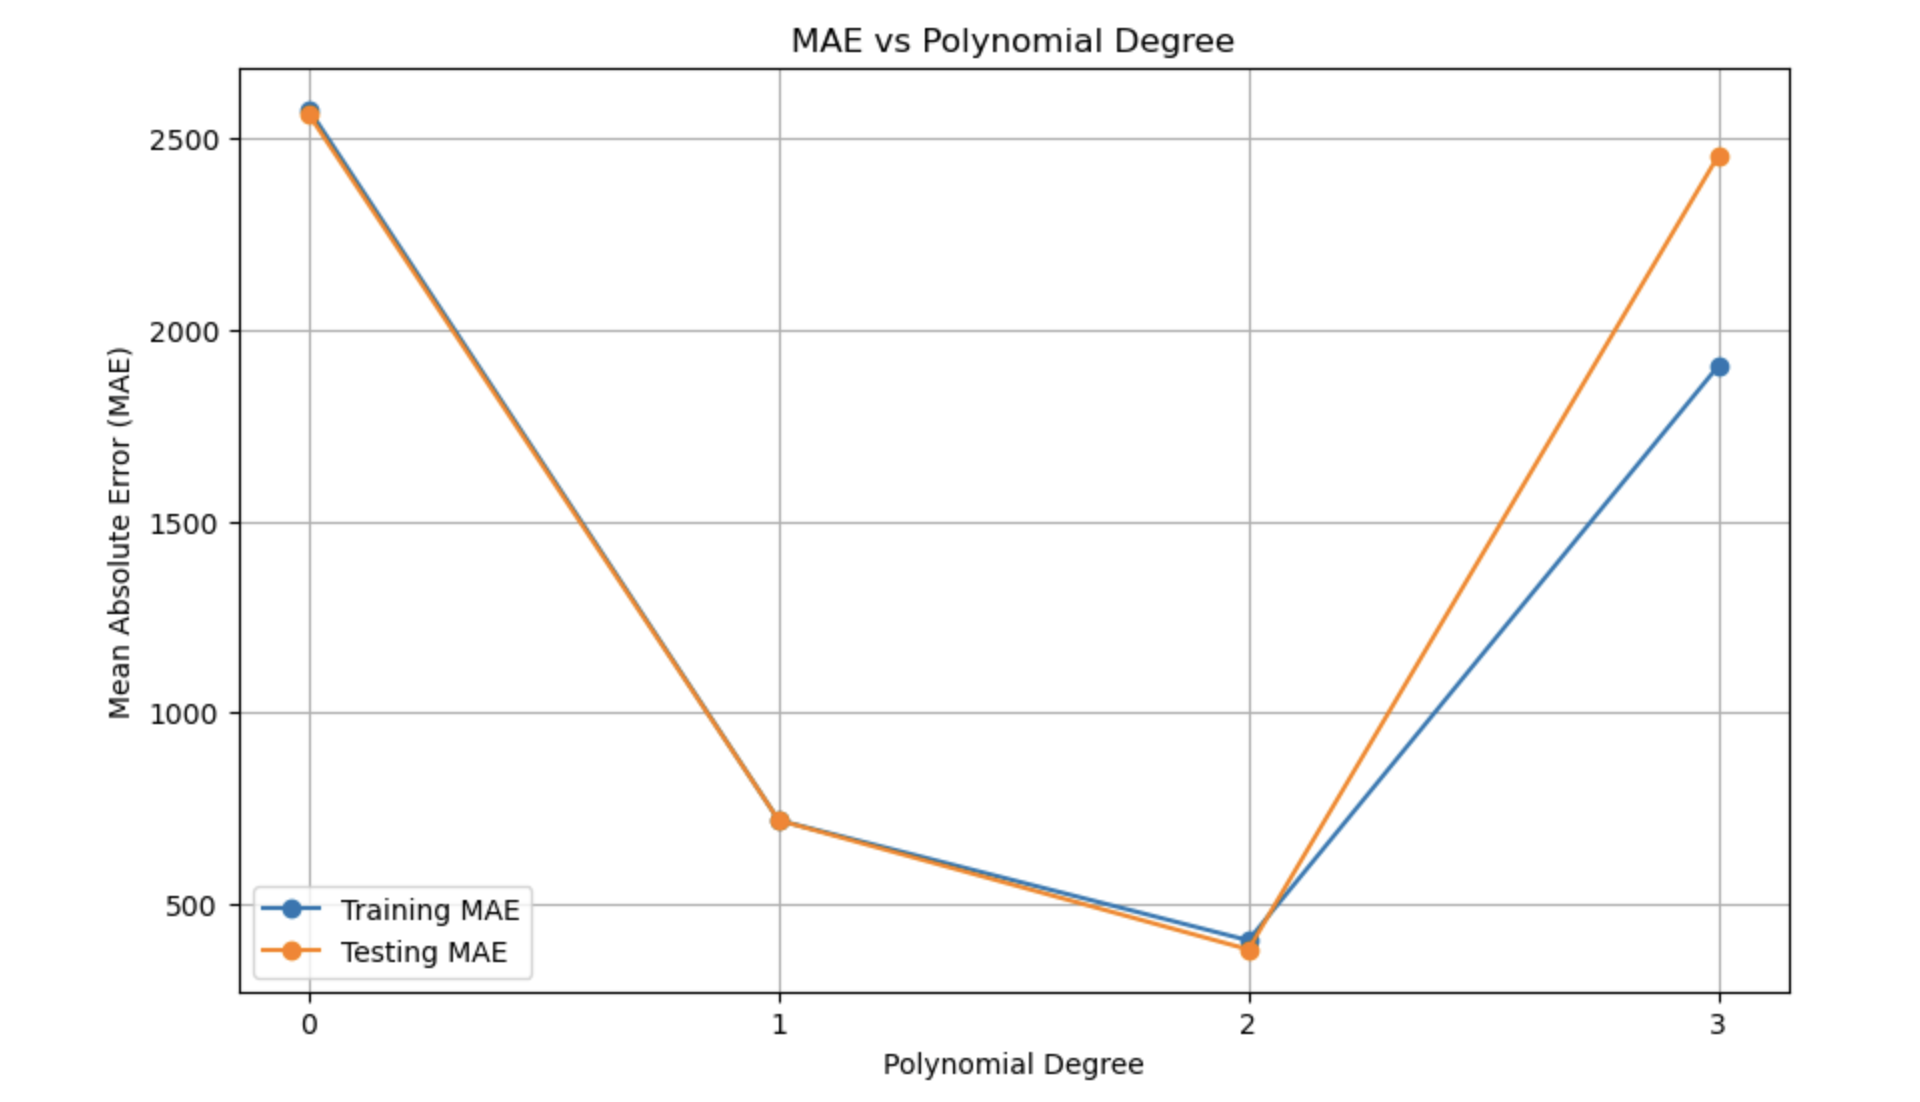
\includegraphics[width=0.8\linewidth]{mae_poly.png} % Replace "example-image" with the filename of your image
    \caption{Mean Absolute Error (MAE) on Training/Testing Data vs Degree of Polynomial Regression Model. Lowest train/test error can be see at degree = 2.}
    \label{fig:degree}
\end{figure}

Based on our results in Figure \ref{fig:degree}, we observed that the Mean Absolute Error was the lowest on both training and testing data when the degree of the polynomial model was squared. As we increased the degree to 3, both training and testing errors seemed to rise, indicating that the model might not effectively capture the underlying relationship in this dataset. Thus, our results from cross validation support our findings from the EDA phase that a quadratic relationship is appropriate. We present the performance of our model on the training data from cross-validation, along with training time, below.

\begin{table}[h]
\centering
\caption{Linear vs.\ Polynomial Performance on Training Data}
\begin{tabular}{|c|c|c|c|}
\hline
Method & Mean MSE & Variance MSE & Time \\
\hline
Linear Regression & 1,129,207.421 & 47,218.77 & 0.0075(s) \\
\hline
Polynomial Regression &  9,055,852.513 & 55,599.664 & 0.072 (s) \\
\hline
\end{tabular}
\label{tab:lr_trn}
\end{table}

Our findings from model training reveal that polynomial regression, particularly with a squared degree, yields a much higher average training error (and variance) compared to the linear regression model across the 5-fold cross-validation. Additionally, polynomial regression incurs a significant increase in computational cost, with its training time nearly ten times longer than that of linear regression. Despite both algorithms having relatively quick training speeds due to their overall simplicity as compared to the other models, the substantial computational overhead of polynomial regression underscores the need to carefully weigh its benefits in capturing non-linear relationships against the associated computational demands. We will also evaluate its performance on the test set and compare with other models below. 

\subsection{Decision Trees}

To determine the optimal set of hyperparameters, we conducted a 5-fold cross-validation procedure on our training data for both the Random Forest and XGBoost models. The table below presents the optimal hyperparameter settings for the Random Forest algorithm, selected from the parameter grid proposed earlier:

\begin{table}[H]
\centering
\caption{Optimal Hyperparameter for Random Forests}
\begin{tabular}{|c|c|}
\hline
Hyperparameter & Optimal Value \\
\hline
Bootstrap & TRUE \\
\hline
Max Depth & None \\
\hline
Max Features & 'sqrt' \\
\hline
Min Samples Leaf & 2 \\
\hline
Min Samples Split & 2 \\
\hline
N Estimators & 10 \\
\hline
\end{tabular}
\label{tab:rf_hyper}
\end{table}

\emph{Random Forests} displays the optimal hyperparameters, providing insight into the Random Forest algorithm’s structure (i) Bootstrap sampling ('Bootstrap = TRUE') diversifies training datasets for each tree. (ii) The absence of a maximum depth ('Max Depth = None') allows trees to grow deep and simplifies decision boundaries. (iii) Features are randomly sampled at each split ('Max Features = sqrt'). (iv) Both leaf and internal nodes require a minimum of 2 samples ('Min Samples Leaf = 2' and 'Min Samples Split = 2'). (v) Utilizing 10 trees ('N Estimators = 10') enables capturing feature interactions. This combination of hyperparameters should enable the Random Forest algorithm to achieve accurate generalization while also potentially mitigating overfitting.

\begin{table}[H]
\centering
\caption{Optimal Hyperparameter for XGBoost}
\begin{tabular}{|c|c|}
\hline
Hyperparameter & Optimal Value \\
\hline
Colsample\_byTree & 0.8 \\
\hline
Gamma & 0 \\
\hline
Learning Rate & 0.1 \\
\hline
Max Depth & 6 \\
\hline
Reg Alpha & 0 \\
\hline
N Estimators & 200 \\
\hline
Reg Lambda & 0.1 \\
\hline
Subsample & 1.0 \\
\hline
\end{tabular}
\label{tab:xg_hyper}
\end{table}

\emph{XGBoost}: Table \ref{tab:xg_hyper} displays the optimal hyperpa-
rameters, providing insight into the XGBoost algorithm’s structure. Using gradient boosting, XGBoost sequentially builds trees to correct errors. (i) Features are sampled at 80\% per tree ('Colsample\_byTree = 0.8') to reduce overfitting. (ii) We put constraints on overall complexity with a maximum depth of 6 ('Max Depth = 6'). (iii) Regularization terms, gamma (set to 0) and lambda (set to 0.1) help control overfitting. (iv) By employing a learning rate of 0.1 ('Learning Rate = 0.1'), each tree's contribution is shrunk to enhance generalization. (v) With 200 boosting rounds ('N Estimators = 200'), model performance iteratively improves. With this combination of hyperparameters, the algorithm should provide accurate results on test data while ensuring robustness.

\emph{Training Accuracy} The table below displays accuracy measures on the training data using 5 fold cross validation, along with the training time. 

\begin{table}[H]
\centering
\caption{Random Forests vs.\ XGBoost on Training Data}
\begin{tabular}{|c|c|c|c|}
\hline
Method & Mean MSE & Standard Deviation & Training Time \\
\hline
Random Forests & 232,322.902 & 17741.65 & 0.453(s) \\
\hline
XGBoost & 171,332.011 & 18,084.45 & 0.254(s) \\
\hline
\end{tabular}
\label{tab:dt_trn}
\end{table}

Table \ref{tab:dt_trn} displays the average training accuracy measures of Random Forests and XGBoost, alongside their respective training times. Notably, both algorithms achieved significantly lower training errors compared to the regression models. Random Forests exhibit a mean MSE of 232,322.902 with a standard deviation of 17,741.65, while XGBoost achieves a lower mean MSE of 171,332.011 with a standard deviation of 18,084.45. Additionally, XGBoost demonstrates a shorter training time of 0.254 seconds compared to 0.453 seconds for Random Forests. These results indicate that XGBoost outperforms Random Forests in terms of accuracy while also being computationally more efficient.

\subsection{Neural Network}

Again, we employed a 5-fold cross-validation procedure with an extensive Grid Search approach to identify the optimal set of hyperparameters for our neural network. Here are the results:

\begin{table}[H]
\centering
\caption{Optimal Hyperparameter for Neural Networks}
\begin{tabular}{|c|c|}
\hline
Hyperparameter & Optimal Value \\
\hline
Learning Rate & 0.1 \\
\hline
Epochs & 250 \\
\hline
Batch Size & 256 \\
\hline
Optimizer & RMSProp \\
\hline
Dropout Rate & None \\
\hline
Number of Neurons in Hidden Layer & 64 \\
\hline
\end{tabular}
\label{tab:nn_hyper}
\end{table}

The grid search method presents the architecture of our neural network model. Specifically, the neural network architecture consists of a single hidden layer with 64 neurons, a learning rate of 0.1 for the model convergence, RMSProp optimizer, and no dropout regularization. Note that for this paper, our search was limited on developing an artificial neural network with one hidden layer, and one may choose to add additional layers and deepen this network further. The number of epochs was determined to be 250. To illustrate the training and testing accuracy versus epoch, refer to the figure below.

\begin{figure}[H]
    \centering
    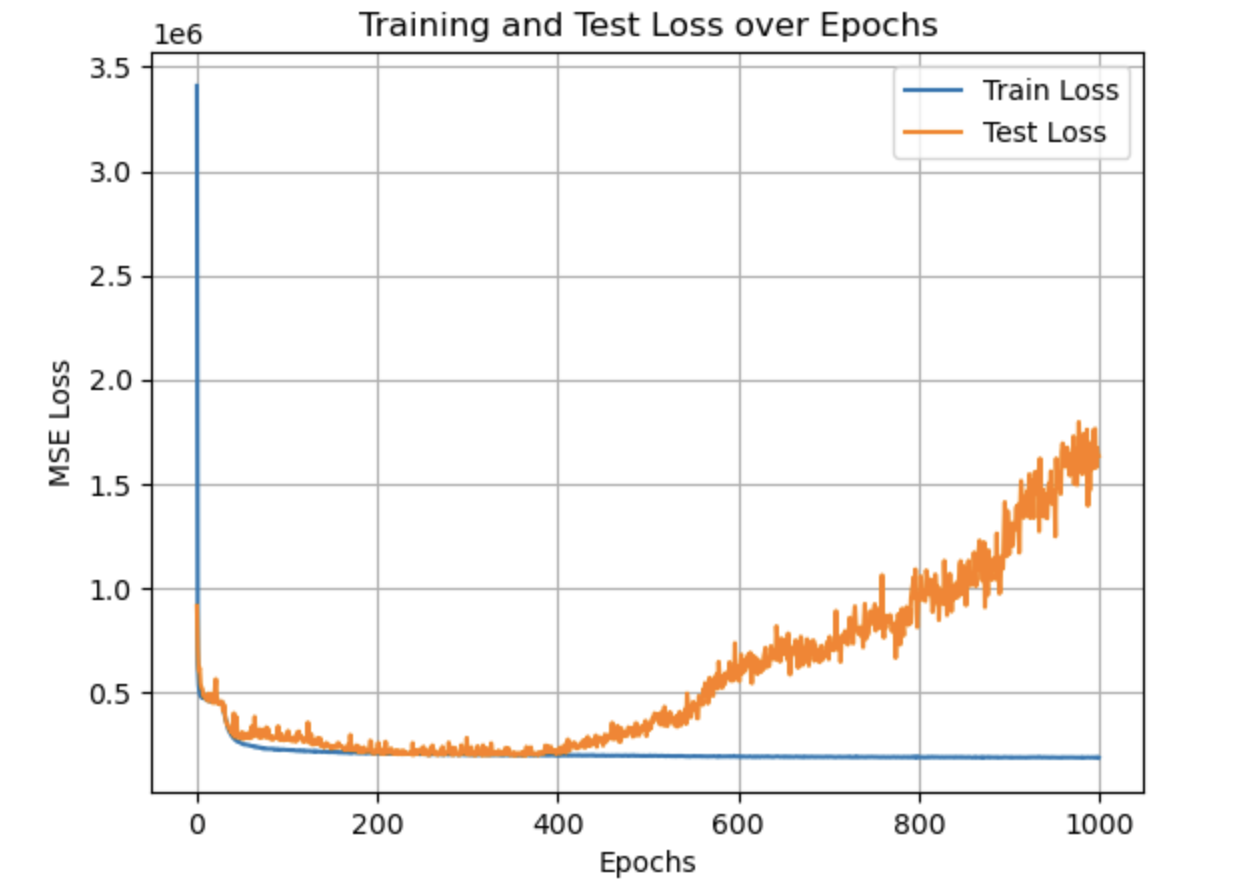
\includegraphics[width=1\linewidth]{1000.png} % Replace "example-image" with the filename of your image
    \caption{Error (MSE) vs Number of Epochs: The figure depicts the training and testing errors as a function of the number of epochs (1000). Overfitting becomes apparent after Epoch 450, as shown by an increase in testing error while the training error remains low.}
    \label{fig:trn-tst-1000}
\end{figure}

We trained the neural network model using the optimal set of hyperparameters across 1000 epochs to learn the weights and observe when the model begins to overfit our data. Figure \ref{fig:trn-tst-1000} suggests that overfitting occurs after epoch 450. Initially, both the training and testing errors significantly decrease as the model weights are learned iteratively. However, around 500 epochs, our neural network model begins to overfit the data: the testing error starts to increase significantly while the training error continues to decrease. This suggests that early stopping training at around 250 epochs can help prevent overfitting.

\begin{figure}[H]
    \centering
    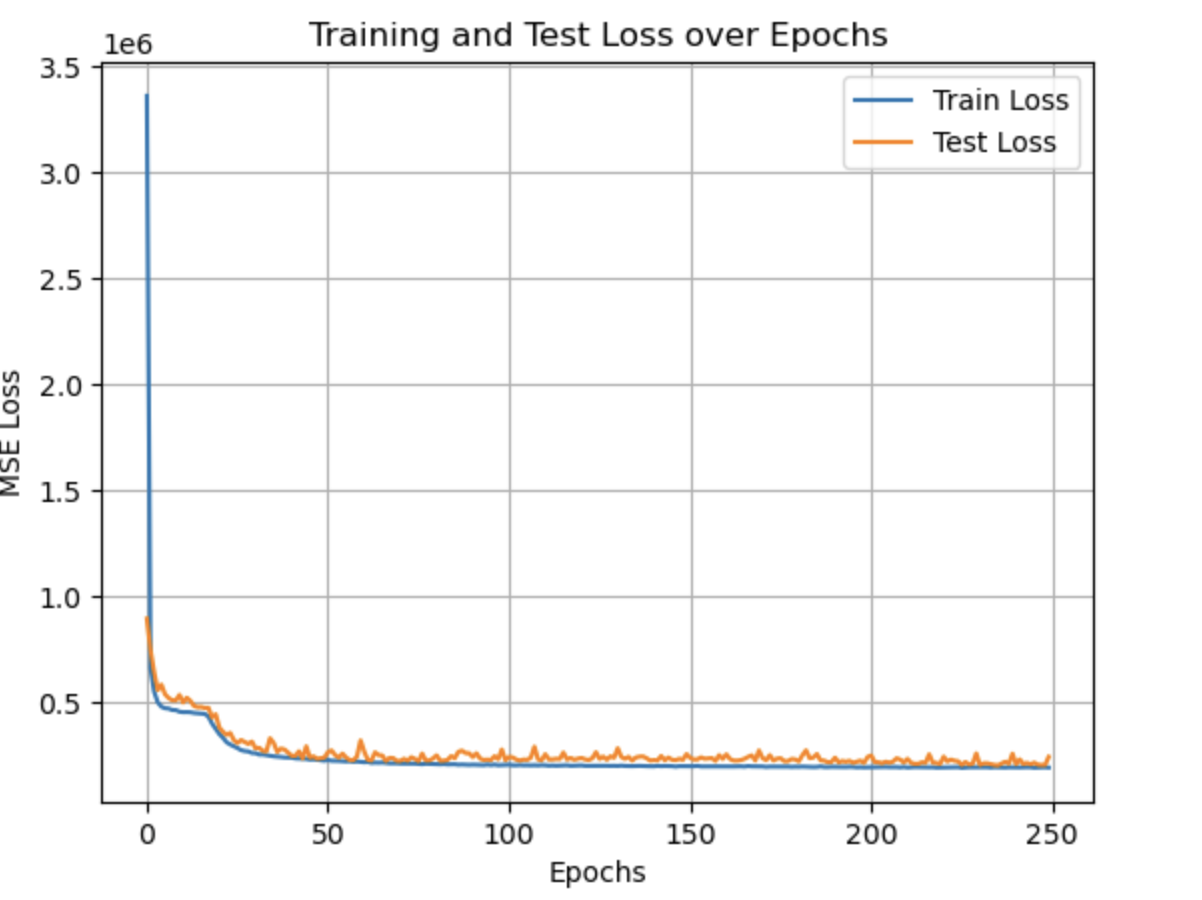
\includegraphics[width=0.8\linewidth]{250.png} % Replace "example-image" with the filename of your image
    \caption{Error (MSE) vs Number of Epochs: The figure depicts the training and testing errors as a function of the number of epochs (250). Both training and testing errors remain low across the 250 epochs.}
    \label{fig:trn-test-250}
\end{figure}

Thus, Figure \ref{fig:trn-test-250} displays that 250 epochs is a suitable choice for our application. We now present the training accuracy and time on this training data. 

\begin{table}[H]
\centering
\caption{Neural Network Performance on Training Data}
\begin{tabular}{|c|c|c|}
\hline
Method & MSE & Training Time \\
\hline
Neural Network & 198,675.7 & 25.3 (s)  \\
\hline
\end{tabular}
\label{tab:mytable}
\end{table}

Based on our training data and the given optimal set of hyperparameters, the neural network model performs quite well on the training data with an MSE of 198,675.7. This MSE ranks as the second best, following XGBoost, and displays better predictive performance as compared to the regression models. However, notably, this model incurred a significantly longer training time of 25 seconds as compared to the other models. Thus, we gain insight into the performance of this model on the original training data. Next, we will examine the model's performance on the test set and compare overall results among the models.

\subsection{Comparison of models on testing data}

The table below displays the performance of each algorithm we've taken from above on the testing data:

\begin{table}[H]
\centering
\caption{Performance of Algorithms on Testing Data: MSE, MAE, $R^2$}
\begin{tabular}{|c|c|c|c|c|}
\hline
Method & MSE & MAE & $R^2$ \\
\hline
Linear Regression & 1,110,908.273 & 718.843 & 0.898 \\
\hline
Polynomial Regression & 459,504.630 & 381.455 &  0.958 \\
\hline
Random Forests & 210,230.72 & 246.879 & 0.9808  \\
\hline
XGBoost & 166,912.918 & 223.123 & 0.984 \\
\hline
Neural Networks & 188,9781.85 & 271.621 & 0.8280 \\
\hline
\end{tabular}
\label{tab:mytable}
\end{table}

The performance of each algorithm on the testing data presents intriguing insights. Linear regression, which served as a baseline model, exhibits the highest MSE and MAE among all algorithms. This suggests the limitation of linear regression in capturing the complexity of relationships between diamond pricing and its characteristics. Polynomial regression performs better, significantly reducing the MSE and indicating its ability to capture non-linear relationships present in the data. Interestingly, despite having a higher training MSE, our polynomial regression model outperforms linear regression in terms of all three metrics on the testing data. This suggests that the inherent quadratic relation observed during the EDA phase in figure \ref{fig:scatter} might indeed be present. Furthermore, both linear and polynomial regression models have the shortest training times, which could be advantageous given limited computational resources.

Both decision tree methods Random Forests and XGBoost demonstrate substantial improvements in performance, achieving significantly lower MSE and MAE values along with higher $R^2$ scores. This suggests that ensemble methods excel in capturing the intricate patterns in diamond pricing, likely due to their ability to model complex interactions between features. In particular, we can see that XGBoost stands out for its superior predictive accuracy and $R^2$ scores as compared to the other models. The training complexity of these models lies between that of linear/polynomial regression and neural networks, and they offer superior performance on the testing data.

Comparatively, the neural network model yields low MSE and MAE, though its coupled with a slightly lower $R^2$ score compared to the ensemble methods. This indicates slightly suboptimal performance on the testing data as compared to those methods. Despite its potential to capture complex relationships, the neural network may require further optimization or a more sophisticated architecture to achieve better results in predicting diamond prices. Additionally, the training time for neural networks is the highest, which could lead to computation scarcity if the model becomes more complex or if more training data is added.

Overall, Random Forests and XGBoost emerge as the top performers on the testing data, showcasing their effectiveness in accurately predicting diamond prices. These models, with their capability to handle non-linear relationships and capture intricate patterns, offer valuable insights into the factors influencing diamond pricing and can guide pricing strategies and market analyses effectively.

\section{Conclusion}

In this study, we investigated various machine learning algorithms to predict diamond prices based on key characteristics such as carat, cut, color, clarity, and dimensions. Our analysis demonstrated that advanced machine learning techniques, particularly Random Forests, XGBoost, and neural networks, significantly outperformed traditional linear regression models in terms of predictive accuracy.

The exploratory data analysis revealed that carat is the most influential feature, showing strong correlations with price and other dimensions. Our findings suggest that leveraging these advanced models can provide jewelers and consumers with more accurate pricing, enhancing decision-making and market transparency.

Overall, Random Forests and XGBoost emerged as the top performers, showcasing their effectiveness in handling non-linear relationships and capturing intricate patterns in the data. The neural network model also showed promise, though it requires further optimization to reach its full potential. Linear and polynomial regression models, while simpler and faster to train, were less effective in capturing the complexities of diamond pricing. By adopting robust machine learning methodologies, the diamond industry can benefit from more precise pricing strategies, leading to improved market efficiency and customer satisfaction.

\subsection{Potential for Future Efforts}

Future research can build on these findings by incorporating a larger dataset to capture more diverse patterns and improve model generalization, conducting a more comprehensive grid search with a larger hyperparameter space to find optimal settings for models, particularly neural networks, and integrating additional features such as market trends, regional price variations, and other economic indicators to enhance model accuracy. Further optimization of neural network architectures, such as experimenting with deeper networks and different types of layers, could improve performance. Additionally, applying these models to other diamond datasets can validate their generalizability and overall robustness. We can continue to refine and expand upon the models and methodologies used in this study, and the diamond industry can further enhance its pricing strategies and decision-making processes.

\section{Project Road-Map}

To conclude, our project involves a regression-supervised learning task to predict the price of a diamond based on several different features. Our machine learning pipeline involved several steps: (i) \textbf{Exploratory Data Analysis (EDA):} During the first three weeks, our group focused on the exploratory data analysis portion. This took about 3-4 weeks. We began by plotting the distribution of our features to understand the spread of our data and account for potential skewness. Since outliers can significantly affect the overall accuracy of machine learning models, we used various outlier detection techniques, including the IQR computation, to identify and remove them. Our group contributed equally to this component: Andrew and Yifan focused on outlier detection, while Aditya, Eshan, and Nandini worked on creating the plots. (ii) \textbf{Model Implementation:} During the next three weeks, we implemented various models. Aditya worked on implementing the decision tree models and performed the necessary grid search for hyperparameter tuning. Andrew and Yifan focused on the neural network and regression models. This process took about three weeks (weeks 4-8 of the quarter). This step was the most rigorous and time consuming, as we evaluated each of the models against one another and tested many variations of hyperparameter spaces to find the optimal set in our application. During this time, Aditya also began writing the final report to ensure we stayed on schedule. (iii) \textbf{Report Writing:} The paper was written over the course of the quarter, once model training was completed to some extent. In weeks 9-10, the team finished the paper together. (iv) \textbf{Final Touches:} During the final week, we implemented finishing touches on the project report and integrated the model weights into the project GUI. Nandini and Eshan handled the HTML connections. Overall, our project demonstrated the importance of accurate diamond price prediction and showcased the effective use of machine learning models in achieving this goal.

\textbf{Group Contributions:} The group had equal contributions throughout the course of this project. Andrew, Yifan, and Aditya focused on the model training and writing the paper. Nandini and Eshan worked on exploratory data analysis, setting up the Github repo, and creating the Project GUI environment for users. Aditya remained in contact with the TA and professors to ensure the groups needs were met and all inquiries we resolved in a timely manner. 

The \textbf{Github repository} for our project may be found here: https://github.com/adimittal03/ECS171-Final-Group21. 



\newpage
\begin{thebibliography}{00}
\bibitem{kino} Kino, S., Hsu, Y.-T., Shiba, K., Chien, Y.-S., Mita, C., Kawachi, I., and Daoud, A. (2021). A scoping review on the use of machine learning in research on social determinants of health: Trends and research prospects. SSM - Population Health, 15, 100836.
\bibitem{sarker} Sarker, I.H. Machine Learning: Algorithms, Real-World Applications and Research Directions. SN COMPUT. SCI. 2, 160 (2021). https://doi.org/10.1007/s42979-021-00592-x
\bibitem{Alsuraihi} Alsuraihi, W., Al-hazmi, E., Bawazeer, K., \& AlGhamdi, H. Machine learning algorithms for diamond price prediction. In Proceedings of the 2020 2nd International Conference on Image, Video and Signal Processing, 150–154 (2020).
\bibitem{Mamonov} Mamonov, S. \& Triantoro, T. Subjectivity of diamond prices in online retail: Insights from a data mining study. J. Theor. Appl. Electron. Commer. Res. 13(2), 15–28 (2018).
\bibitem{Pandey} Pandey, A. C., Misra, S., \& Saxena, M. Gold and diamond price prediction using enhanced ensemble learning. In 2019 Twelfth International Conference on Contemporary Computing (IC3), 1–4 (IEEE, 2019).
\bibitem{Scott} Scott, F. \& Yelowitz, A. Pricing anomalies in the market for diamonds: Evidence of conformist behavior. Econ. Inq. 48(2), 353–368 (2010).
\bibitem{Kutner}Michael Kutner, Christopher Nachtsheim, John Neter, and William Li. Applied Linear Statistical Models. 1974.
\bibitem{Seber}Seber, G. A. F., \& Lee, A. J. (2012). Linear Regression Analysis. Hoboken, NJ: John Wiley \& Sons.
\bibitem{Wright} Wright, John T. "Linear Regression Analysis." British Medical Journal, vol. 310, no. 6977, 1995, pp. 1120-1124. BMJ Group
\bibitem{Weisberg} Weisberg, S. (2005). Applied Linear Regression. Wiley.
\bibitem{Breiman} Breiman, L. (2001). Random forests. Machine Learning, 45(1), 5-32.
\bibitem{Chen} Chen, T., \& Guestrin, C. (2016). XGBoost: A Scalable Tree Boosting System. In Proceedings of the 22nd ACM SIGKDD International Conference on Knowledge Discovery and Data Mining (pp. 785-794).
\bibitem{LeCun} LeCun, Y., Bengio, Y., \& Hinton, G. (2015). Deep learning. Nature, 521(7553), 436-444.
\bibitem{Rumelhart} Rumelhart, D. E., Hinton, G. E., \& Williams, R. J. (1986). Learning representations by back-propagating errors. Nature, 323(6088), 533-536.
\bibitem{Bergstra} Bergstra, J., \& Bengio, Y. (2012). Random search for hyper-parameter optimization. Journal of Machine Learning Research, 13(Feb), 281-305.
\bibitem{us} U.S. jewelry market size and share: Industry Report, 2030. U.S. Jewelry Market Size And Share | Industry Report, 2030. (n.d.). https://www.grandviewresearch.com/industry-analysis/us-jewelry-market-report
\bibitem{diamond} Diamond Jewelry Market Size \& Share Analysis Report, 2030. (n.d.). https://www.grandviewresearch.com/industry-analysis/diamond-jewelry-market-report
\bibitem{kaggle} Agrawal, S. (2017a, May 25). Diamonds. Kaggle. https://www.kaggle.com/datasets/shivam2503/diamonds
\bibitem{Bottou} Bottou, L. (2010). Large-Scale Machine Learning with Stochastic Gradient Descent. In Proceedings of COMPSTAT'2010, Springer. DOI: 10.1007/978-3-7908-2604-3\_16
\bibitem{Kingma} Kingma, D. P., \& Ba, J. (2015). Adam: A Method for Stochastic Optimization. In International Conference on Learning Representations (ICLR). URL: https://arxiv.org/abs/1412.6980
\bibitem{Tieleman} Tieleman, T., \& Hinton, G. (2012). Lecture 6.5 - RMSProp: Divide the gradient by a running average of its recent magnitude. COURSERA: Neural Networks for Machine Learning. URL: https://www.cs.toronto.edu/~tijmen/csc321/slides/lecture\_slides\_lec6.pdf

\end{thebibliography}
\vspace{12pt}


\end{document}
